\documentclass{amia}

\usepackage[utf8]{inputenc} % allow utf-8 input
\usepackage[T1]{fontenc}    % use 8-bit T1 fonts
\usepackage{hyperref}       % hyperlinks
\usepackage{url}            % simple URL typesetting
\usepackage{booktabs}       % professional-quality tables
\usepackage{amsfonts}       % blackboard math symbols
\usepackage{nicefrac}       % compact symbols for 1/2, etc.
\usepackage{microtype}      % microtypography
\usepackage[super]{nth}     % JK: for 1st-ing and 2nd-ing
\usepackage{graphicx}       % added by seth - image support
\graphicspath{ {./images/} }
\usepackage{footmisc}       % better footnote support

\usepackage{hyperref}
\hypersetup{
    colorlinks=true,
    linkcolor=blue,
    filecolor=magenta,
    urlcolor=blue,
    citecolor=blue
}
 
\urlstyle{same}

\renewcommand{\thefootnote}{\alph{footnote}}

\begin{document}

\title{%
  Kung Faux Pandas \\
  \large Simplifying privacy protection
  }

\author{
  James King MIDS$^{1}$\footnote{Authors JK and SR contributed equally to this work\label{contribution}},
  Seth Russell MS$^{1}$\footref{contribution},
  Tellen D. Bennett, MD, MS$^{1,2}$,\\
  Debashis Ghosh, PhD$^{1,3}$
  }
  
\institutes{
  $^1$CU Data Science to Patient Value (D2V), Anschutz Medical Campus, Aurora, CO;
  $^2$Pediatric Critical Care, University of Colorado School of Medicine, Aurora, CO;
  $^3$Biostatistics and Informatics, Colorado School of Public Health, Aurora, CO\\
}

\maketitle

\noindent{\bf Abstract}

\textit{There are many barriers to data access and data sharing, especially in the domain of computational research using health care data. Legal constraints, such as HIPAA, protect patient privacy but slow access to data and limit reproducibility. We provide a description of an end-to-end system called \emph{Kung Faux Pandas} for easily generating de-identified or synthetic data which is statistically similar to real data but lacks sensitive information. This system focuses on data synthesis and de-identification narrowed to a specific research question to allow for self-service data access without the complexities required to generate an entire population of data that is not needed for a given research project. Kung Faux Pandas is an open source publicly available\footnote{\url{https://github.com/CUD2V/kungfauxpandas}} system that lowers barriers to HIPAA- and GDPR-compliant data sharing for enabling reproducibility and other purposes.}

\section{Introduction}

Independent reproduction and replication of results are critical components of scientific inquiry. Barriers to data access and sharing are the most important impediments to reproducibility in health data science research. Health care research has unique challenges because of necessary personal data privacy protections.

Several methods exist to de-identify (remove key identifiers, group individuals, and related anonymization techniques \cite{hippapro}) and synthesize data (create data through algorithmic means, population level statistics, randomization, ideally with preservation of multivariate relationships between records \cite{walonoski_synthea_2018, patki_synthetic_2016, choi_generating_2017}). However, no pipeline currently exists with which computational investigators can routinely \emph{anonymize} or \emph{synthesize} data to facilitate access and sharing. This work addresses that gap.

We have created an open source software library called \emph{Kung Faux Pandas (KFP)} which allows for the modular combination of established privacy protection methods with the popular Python Pandas data science library\cite{mckinney-proc-scipy-2010}. KFP also provides a Structured Query Language (SQL) interface which enables users to query a database and receive a data set without personal information through either anonymization or synthetic data generation.

\section{Background}

Recent work has clarified the definition and importance of reproducibility and a closely related concept, replicability. Leek and Peng have defined reproducibility as the "ability to recompute data analytic results given an observed dataset and knowledge of the data analysis pipeline," and replicability as "the chance that an independent experiment targeting the same scientific question will produce a consistent result."\cite{leek_opinion_2015,peng_reproducible_2006} Others have used the terms in a reverse fashion\cite{drummond_replicability_2009}. Despite the semantic differences, there is broad agreement that an independent experiment with confirmatory results is the strongest support of any experiment. One early influential paper on the topic of reproducibility in scientific computing lists the key factors in reproducibility as: available data, input parameters, documentation, software code, and an environment capable of running the provided software code. These items are difficult to completely convey in a traditional research paper \cite{schwab_making_2000}.

In the context of machine learning (ML), sufficient detail is required such that an independent investigator could create the same hardware and software configuration, data used for all experiments, source code, documentation on data and how to run/configure software, and tests that verify the software runs correctly. Once a result can be reproduced, new researchers can then build upon the methods, gather new data for testing/validation, or discover alternative methods to replicate a result.

Many domains in which health data science investigators work have legal barriers that make it difficult to enable independent verification of ML models which frequently require enormous amounts of training data. As an example, in the health care domain in the United States, a key law governing health data is the Health Insurance Portability and Accountability Act (HIPAA). HIPAA is backed by significant civil penalties as well as specifics about data security and what can and cannot be done with protected health information \cite{hippaviol}. While there are other domain specific data privacy laws, there are also some broad rules that affect entire countries such as the European Union's General Data Protection Regulation (GDPR). The GDPR puts in place new rules about data ownership and control in an attempt to give individuals more control over their information.

The current legal environment creates a difficult situation for scientists in the health care domain. Early examples of re-identification attacks \cite{sweeney_2002} have created apprehension on the part of businesses and legal experts in data sharing \cite{ohm_broken_2009}. Getting access to source health care data is slow and isn't always granted \cite{hodge_legal_1999, committee_hipaa_privacy_rule_2009}. More recently, research in the data sharing/privacy protection space has focused more on synthesis techniques such as in the case of the Synthea system, a tool to generate an entire outpatient Electronic Health Record (EHR) based on population statistics \cite{walonoski_synthea_2018}. Current solutions are not without their drawbacks however as they frequently require significant configuration of metadata before they can generate data or they attempt to solve the entire solution space and consequently are very slow to run.

\section{System Details}

One way around the difficulties of source data access is to separate the dependency between data and analysis in such a way that analysis can be performed without the analyst having access to the source data. Such a process can be possible if a sufficiently detailed description of the sensitive data is provided. Appropriate models can be developed and initially validated before either being handed off to a data custodian who then runs the processes on protected data and returns the results to the researcher or access to the protected data has been granted directly to the researcher. Solutions of this form have been possible for some time, but are awkward in practice because activities such as data cleaning, exploration, and model building are interactive and iterative processes that require more than just descriptions of data.

KFP addresses the issue of data access by generating data that is ``statistically similar'' to the real data but does not itself contain any sensitive data. We collectively refer to de-identified data and synthetic data as \emph{faux-data}. We use the term faux as it is used in the fashion sense of the word: the use of man made materials that look and feel like real leather, fur, etc., but without the problematic derivation from live animals and reliance upon limited resources. This faux-data can be analyzed, cleaned, feature-engineered, etc. as if it were the actual source data. KFP provides a standard mechanism for wrapping a privacy protection method into a plug-in which integrates the method with the Pandas DataFrame model. Two of these plug-ins are provided with full documentation for creating other plug-ins.

As the data generated through KFP has no protected component, it can be shared along with code or methods to improve reproducibility as well as aid in replicability. To further the aim of reproducibility we have provided our code and a randomly generated dataset for testing purposes through our GitHub repository in a range of formats: Python environment files (conda and pip) to allow others to start with the same software libraries and specific versions that we used, a Docker \cite{merkel_docker, docker_website} container with code and sample data installed and already configured, and all source code along with version history so others can follow our development process. Also included in our GitHub repository are unit tests for KFP using the Python library pytest. Unit tests helped to validate correct functioning of KFP and provides a foundation from which to prevent regressions as new features are added. 

KFP focuses on generating faux-data narrowed to a specific subset that a researcher is interested in rather than attempting to generate an entire population of data such as an entire EHR or longitudinal patient record. By focusing on just the data needed, performance is improved, the need for extensive modeling or metadata configuration is reduced, and the amount of faux-data generated and stored is minimized. Although the plugable methods included for faux-data generation have been shown to effectively replace source data for analysis, KFP facilitates a more through process that includes an initial exploration with faux-data followed by a repetition of methods on original source data through query logging and thereby aiding in replication.

\subsection{System Architecture}

Ideally a computational investigator should develop, test, and validate models using all available data. This is most easily accomplished when they have unfettered access to all data in the problem domain they are working in. Figure~\ref{fig:architecture} shows the novel architecture of KFP: data access through an intermediary that can synthesize data on-demand. Items in blue are features of KFP; items in grey or with dashed lines are not provided. KFP is designed to fit into an existing infrastructure with a protected data source secured behind a firewall along with user authentication. 

\begin{figure}[ht]
  \centering
  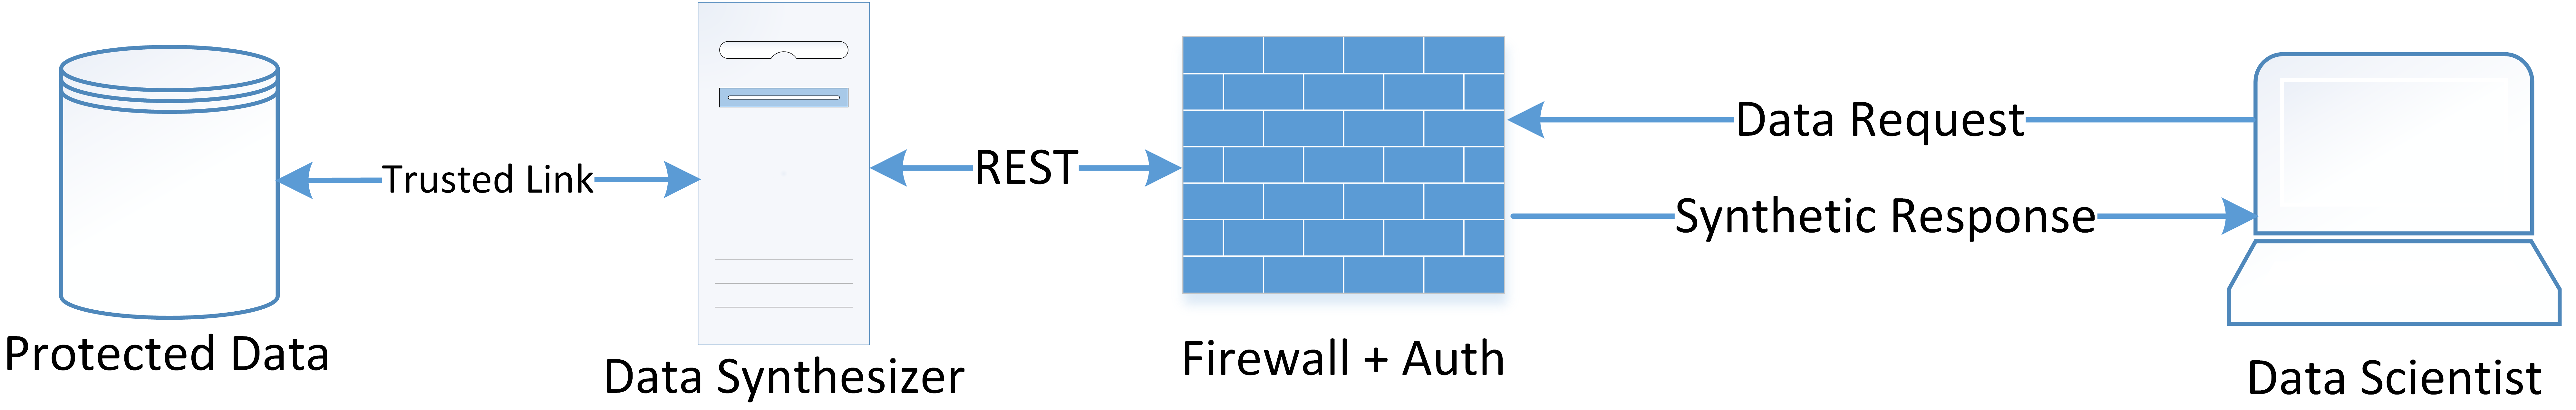
\includegraphics[width=\textwidth]{prototype_architecture}
  \caption{System Architecture.}
  \label{fig:architecture}
\end{figure}

Figure~\ref{fig:synthesis_process} shows the automated faux-data request/response process. Items in grey with dashed lines are not provided by KFP but are either pre-existing or provided by the user. All queries submitted to the system are first pre-processed to remove clauses such as "ORDER BY" which are made ineffective by the synthesis process. All queries are logged for later analysis and results cached to optionally improve synthesis performance for repeated queries. Next the processed query is executed against the protected data set and results are passed into the modular synthesis process. While the current implementation only utilizes a couple of synthesis methods, data scientists or data warehouse owners can insert their own custom method or modify existing methods. For additional details on the modular synthesis processes, see the section "Included Synthesis Methods." Previously removed "ORDER BY" clauses are re-applied to the faux-data before results are returned to the user. Finally, although not implemented in this version of KFP, synthetic results could be held back until reviewed and approved for release by the data owner.

\begin{figure}[ht]
  \centering
  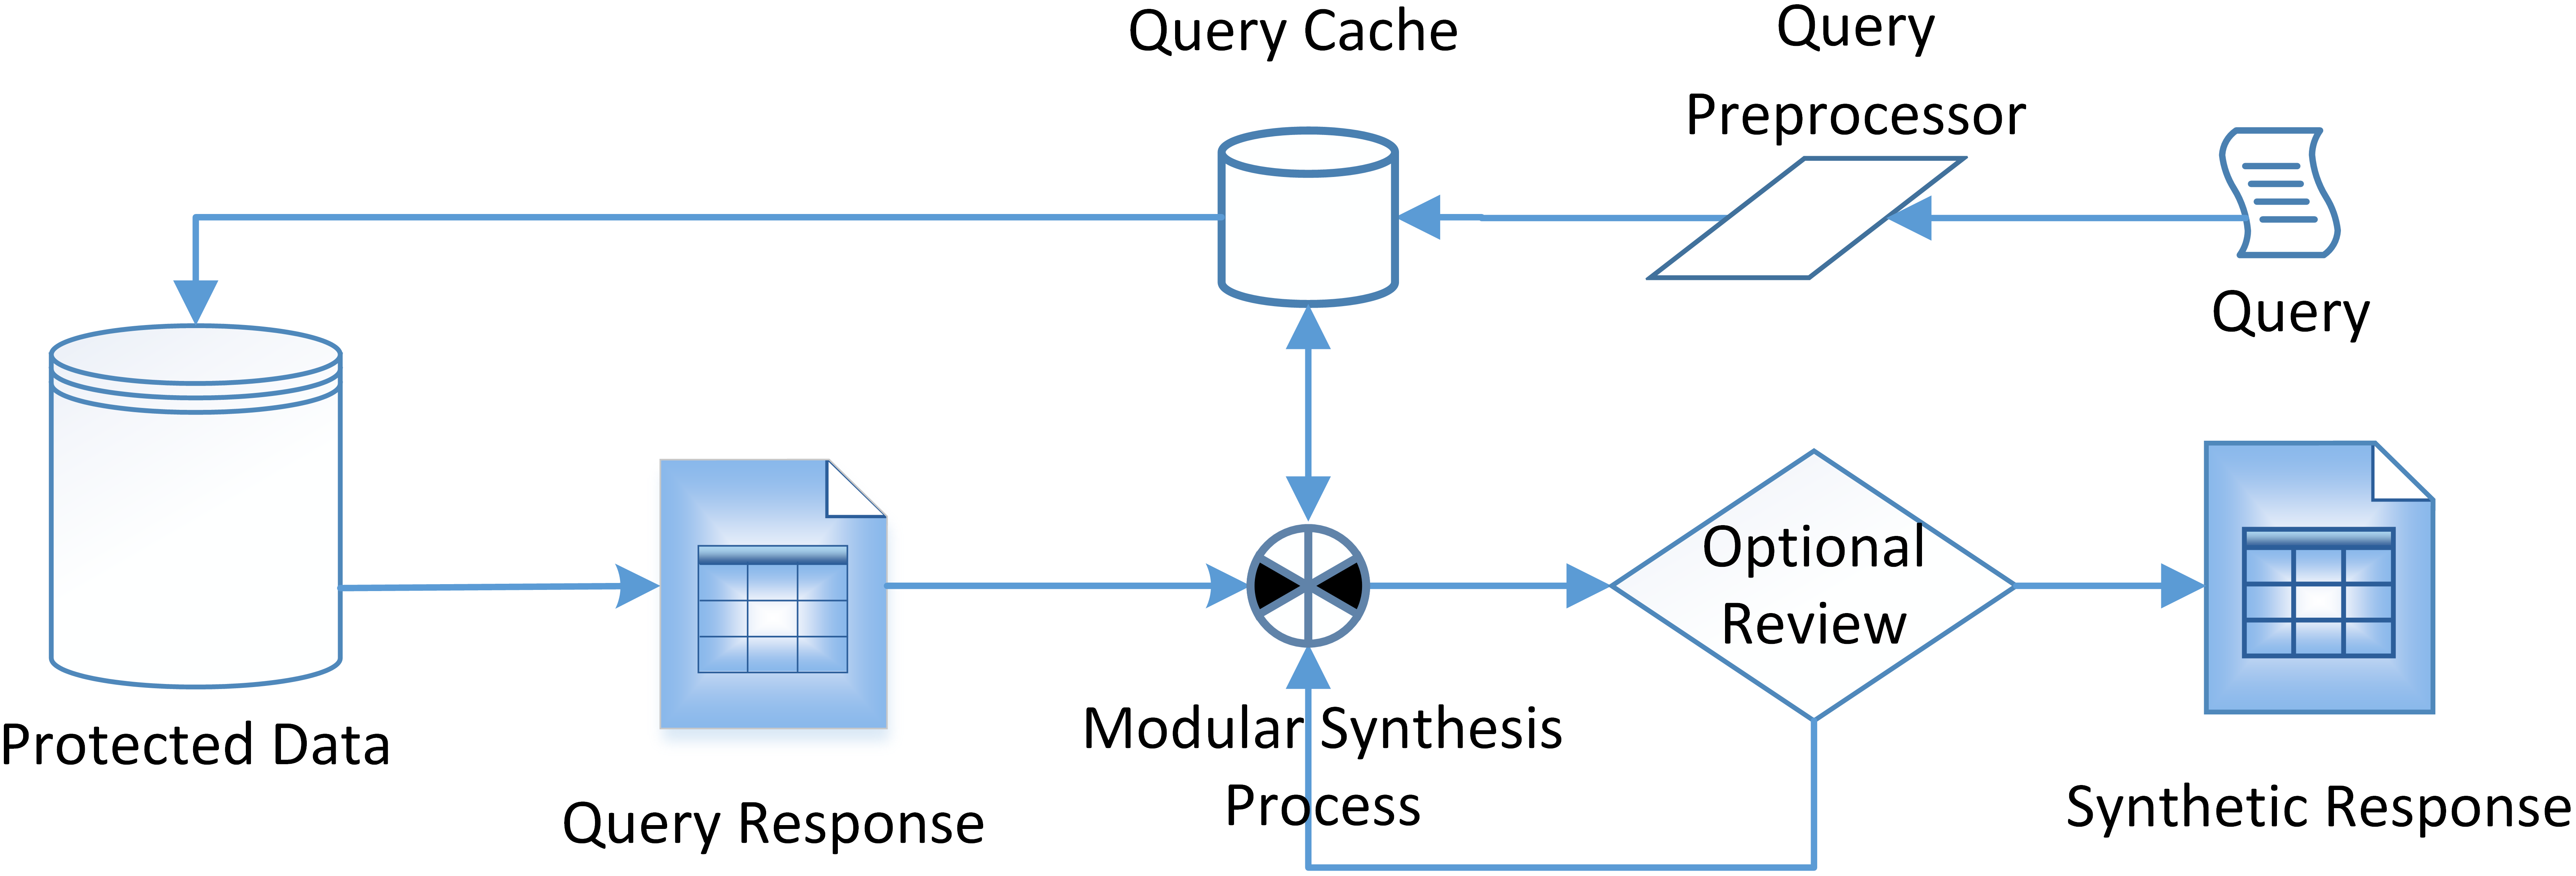
\includegraphics[width=120mm]{data_synthesis_process}
  \caption{Data synthesis process.}
  \label{fig:synthesis_process}
\end{figure}

KFP provides multiple methods by which a health data scientist can access on-demand faux-data. As shown in Figure~\ref{fig:ui}, a single page web application (SPA) allows for users to directly enter SQL queries, submit them to the connected database, and receive faux-data according to the selected generation method. The SPA additionally allows for the upload of csv files (not shown) to allow for ease of evaluation and testing of the provided data synthesis methods. Faux-data can either be viewed directly in browser or downloaded in csv format for use in a health data science process. In order to facilitate querying and understanding of the data model, the database metadata is presented to the user in a collapsible section. The provided Hypertext Transfer Protocol (HTTP) Representational State Transfer (REST) service \cite{w3c_working_group_webservices}, utilized by the SPA, allows for cross language compatible requesting and receiving of faux-data, again via SQL query. Lastly, for Python based software or languages with an interface to Python, the kungfauxpandas.py file and associated classes can be imported and called natively. This Python native API gives full control over all parameters specific each synthesis plugin; the SPA and REST APIs use the default parameters associated with each plugin.

\begin{figure}[ht]
  \centering
  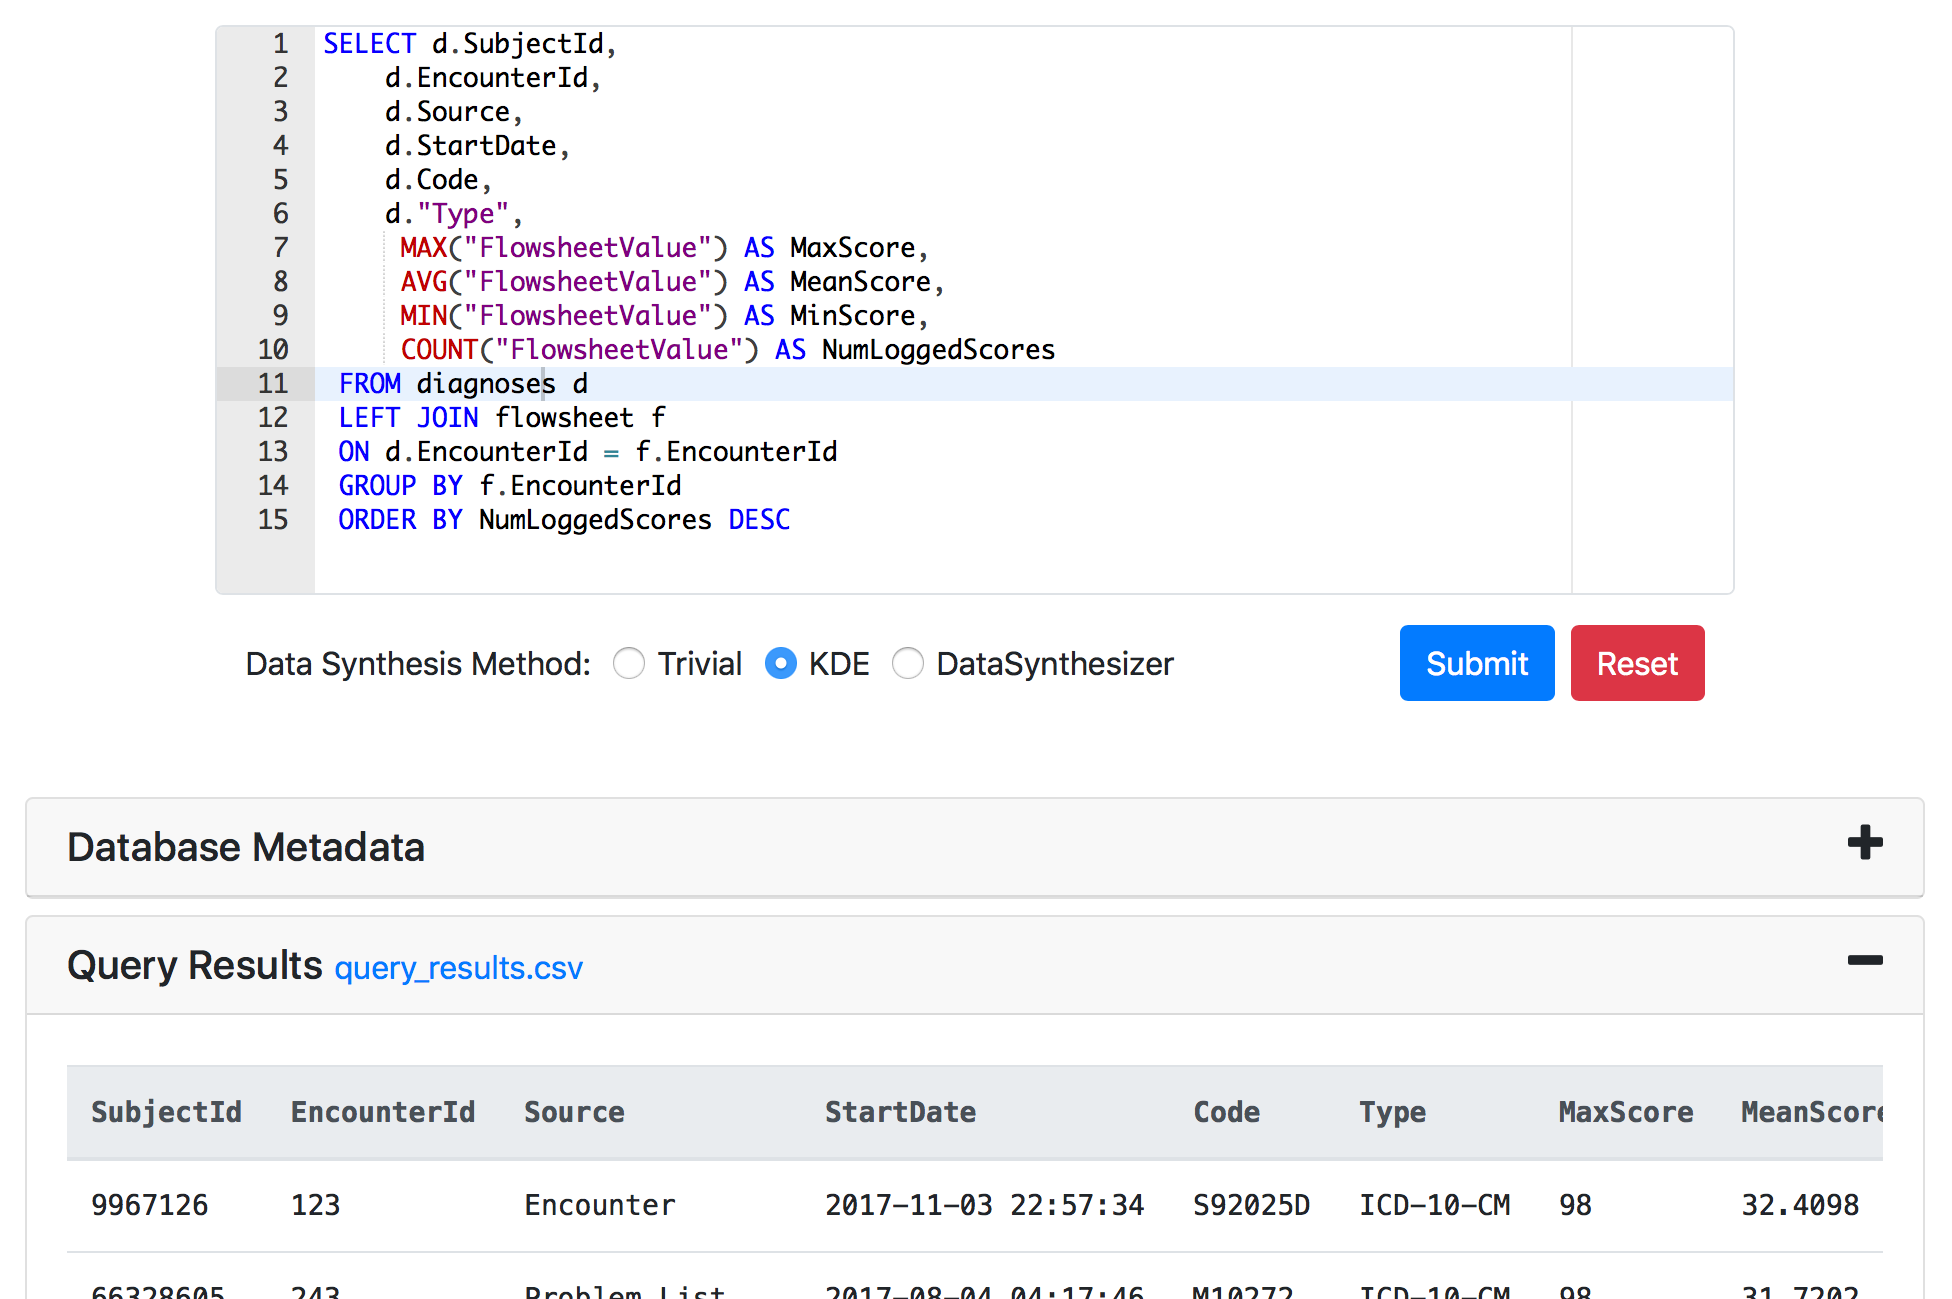
\includegraphics[width=\textwidth]{ui_screenshot3}
  \caption{User Interface.}
  \label{fig:ui}
\end{figure}

\subsection{Included Synthesis Methods}

KFP provides a framework by which any number of methods for data privacy can be carried out. This framework is comprised of a some base classes and methods that can be extended or overridden, several examples of plugins, and unit tests for validation purposes. As of this writing we have implemented two plugins that use different techniques for data synthesis: a kernel density estimator and DataSynthesizer. The kernel density estimator from scipy.stats.gaussian\_kde uses the method developed by Silverman \cite{silverman_density_1986} which handles ordinal and ratio data yet runs quickly on standard consumer level hardware. Two methods for this plugin are provided: an independent attribute mode where each variable is considered in isolation, and a correlated attribute mode where all variables are evaluated and synthesized together on an observation by observation basis. The DataSynthesizer method, created by Ping et al. \cite{ping17datasynthesizer} is built on differential privacy mechanisms and has multiple internal methods for data generation ranging from random generation based on data type to Bayesian modeling of inter-relationships among columns of data. As a result of their methods, the DataSynthesizer offers a unique contribution to the synthetic data generation space: it can work with no configuration other than input data, or can be configured to provide more custom results. In DataSynthesizer, the authors show that the synthetic data generated preserves privacy while still being useful enough for actual data analysis (see also \cite{howe_synthetic_2017}).

\begin{table}
   \caption{Summary of Included Data Synthesis Methods}
   \label{included-methods}
   \centering
   \begin{tabular}{p{12em} l p{20em}}
     \toprule
     Method                                 & Source                    & Notes \\
     \midrule
     %row 1 column 1
     Kernel Density Estimator; independent attribute mode
     %row 1 column 2
     & scipy.stats.gaussian\_kde
     %row 1 column 3
     & Creates a Gaussian Kernel Density Estimator using the Silverman method; fast but doesn’t maintain correlation between variables of the same observation.\\
     %row 2 column 1
     Kernel Density Estimator; correlated attribute mode &
     %row 2 column 2
     scipy.stats.gaussian\_kde &
     %row 2 column 3
     Creates a Gaussian Kernel Density Estimator across all variables per observation using a kde.factor of 0.01 \\
     %row 3 column 1
     DataSynthesizer; independent attribute mode
     %row 3 column 2
     & Ping et al.
     %row 3 column 3
     & A histogram is derived for each attribute, noise is added to the histogram to achieve differential privacy, and then samples are drawn for each attribute; fast but doesn’t maintain correlation between variables of the same observation.\\
     %row 4 column 1
     DataSynthesizer; correlated attribute mode
     %row 4 column 2
     & Ping et al.
     %row 4 column 3
     & Data is generated through a differentially private Bayesian network capturing the correlation between attributes. Computationally expensive and requires larger input dataset compared to independent attribute mode.\\
     \bottomrule
   \end{tabular}
   \vspace{+3mm}
 \end{table}

\section{Experiments}

In this section we evaluate the performance of the KFP plugins to see how closely the methods meet the stated goals of ease of use, similarity to input data, and total time to run. Hardware for these performance and evaluation tests was a 2017 MacBook Pro, 3.1 GHz Intel Core i7, 16GB 2133 MHz LPDDR3 with macOS 10.12.6. KFP software is written in Python 3.6; all packages and dependencies can be installed with identical versions using the provided requirements.txt, environment.yml file, or Docker container. Database queries were run against the relational database PostgreSQL version 9.6.9. Data was generated using the notebook test\_data\_generator.ipynb available in our GitHub repository. The sample data population is composed of 100,000 patient encounters with various dimensions spread across several tables, the largest of which contains 10,539,549 rows of data. The sample query generating the "real" input data is composed of 8 total columns composed of IDs, categorical variables, and floating point numbers.

\subsection{Timing Method}

Table~\ref{timing_results} documents results obtained from running the various plugins. Source code for running these performance tests are available in the Jupyter notebook performance\_tests.ipynb. The "Trivial" method provides a baseline comparison for evaluating the overhead of Pandas and correct input/output of the plugin class and function overloading mechanism; it returns the input data frame unmodified. The KDE methods leveraging scipy.stats.gaussian\_kde act as an example of how to create plugins. Additionally the independent vs correlated KDE methods offer different accommodations for performance with correlated vs non-correlated source data. A couple of DataSynthesizer (abbreviated DS in the table) modes are used to demonstrate performance differences as well as generated synthetic data differences. "Independent" mode generates synthetic data with each attribute being modeled independently from the others. "Correlated" attribute mode finds inter-column relationships to more accurately generate synthetic data. Both DataSynthesizer modes are run with no configuration and again "w/Config" by passing in some column-wise dataset specific configuration.

\begin{table}
	\caption{Kung Faux Pandas data synthesis plugin timings (mean seconds)}
	\label{timing_results}
	\centering
	\begin{tabular}{l c c c c c}
		\toprule 
		Method & 10 rows & 100 rows & 1000 rows & 10000 rows & 100000 rows\\
		\midrule 
		Trivial & 2.5e-06 & 2.3e-06 & 2.3e-06 & 2.2e-06 & 2.2e-06 \\
		KDE Independent & 0.086 & 0.079 & 0.074 & 0.074 & 0.122 \\
		KDE Correlated & 0.017 & 0.021 & 0.027 & 2.43 & 120.8 \\
		DS Independent & 0.044 & 0.050 & 0.103 & 0.268 & 2.608 \\
		DS Independent w/Config & 0.045 & 0.040 & 0.064 & 0.120 & 0.799 \\
		DS Correlated & 0.188 & 1.419 & 3.460 & 16.66 & 159.9 \\
		DS Correlated w/Config & 0.172 & 0.627 & 1.393 & 342.7 & 2124 \\
		\midrule
	\end{tabular}
	\vspace{-4mm}
\end{table}

\begin{figure}[ht]
  \centering
  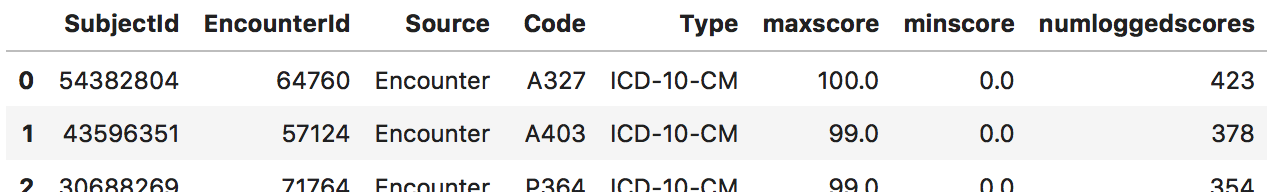
\includegraphics[width=120mm]{sample_source_data}
  \caption{Sample of source data}
  \label{fig:sample_source_data}
\end{figure}
\begin{figure}[ht]
  \centering
  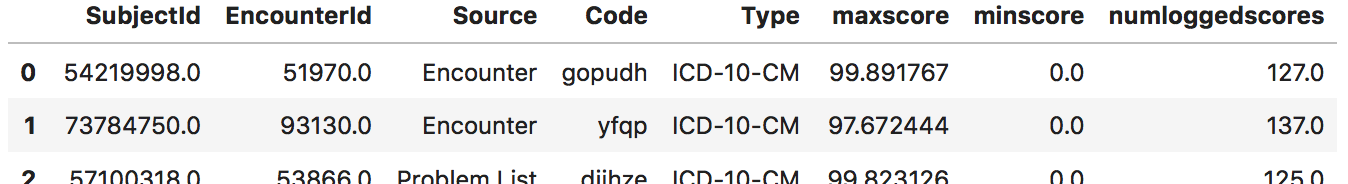
\includegraphics[width=120mm]{sample_synthetic_data}
  \caption{Sample of synthetic data}
  \label{fig:sample_synthetic_data}
\end{figure}

\subsection{Insights}

Figure~\ref{fig:sample_source_data} provides a few rows of the source data for the synthetic plugins. Figure~\ref{fig:sample_synthetic_data} provides a few rows of the synthetic data generated by DataSynthesizer in "Independent" mode.

Fast generation of synthetic data is important in a self-service setting where researchers can generate their own data as needed. As shown in the results, some methods are significantly faster than others as dataset size increases. Another key desire is to have synthetic data be as close as possible to real data without compromising individual privacy. While the KDE plugin is a simple method, it quickly generates data that looks similar to the input data and works well for the range of data types used. DataSynthesizer in "Independent" mode is quick for the tested range of dataset sizes, but without additional configuration, it doesn't generate results that closely match the input dataset. As an example the "Code" column should contain valid International Statistical Classification of Diseases and Related Health Problems, Tenth Revision (ICD-10) codes, but instead has random strings that are similar in length to actual ICD-10 codes that do not line up with values in other columns. The DataSynthesizer "Correlated" attribute mode generates more realistic synthetic data than the "Independent" mode as variables in a single observation that are correlated are modeled together. The "Correlated" method does have a significant larger computational burden when generating synthetic data from larger input dataset sizes.

In all cases, synthetic data generation is a CPU intensive task; no parallelization has been implemented by either KFP nor the plugins used. While memory usage does increase as data size increases, at the 100000 rows seen here, memory usage peaked at around 4.7GB for the Python process.

\section{Discussion}

KFP provides a unique contribution to the space of reproducible computational research. Through providing ad-hoc faux-data, health data scientists can have lower barriers to accessing private data as well as reduced barriers to sharing faux-data derived from private data. Although one clear area for further research would be to develop plugins for additional faux-data methods, there are several areas that go beyond this simple step that could be researched further: improved code sharing of KFP, addressing institutional specific privacy issues, and evaluation of this system in a ML workflow.

While we have provided software code and a description of our methods, we believe that computational reproducibility should go beyond just making source code available. Peng recommends making code available in any form as an excellent first step towards reproducible research; the next step is to make code available "in a durable non-proprietary format" \cite{peng_reproducible_2011}. This is a level of code sharing rarely achieved in computation based research. Currently there is no standard long term format that works for all computational environments. For the Python ecosystem however, the standard for sharing code is via a package on Python Package Index (PyPI). We intend to continue this research to make KFP available as a Python package.

Another area that is open for further research is that of domain and institution specific data privacy needs. In the field of education, statistical methods for calculating sample size based on probability of detecting a specific effect size are commonly used \cite{naep_2009} as the key method for privacy protection. However, it is not clear that these methods are appropriate for general use in ML or domains other than education. Thus, in this work, no attempt has been made to constrain data set sizes nor provide additional proofs of data protection. KFP could be modified to return no results if a minimum threshold is not met or, alternatively, data boosting techniques in combination with data synthesis could be used based on the risk profile of the data owner(s).

The last area recommended for further research is to deploy and observe the use of KFP in an active health data environment where researchers are working with sensitive datasets. A key limitation that may be identified is that of performance characteristics, particularly in a multi-user setting against a large relational database store. Additionally, as no private data was distributed via this system, actual review by security and compliance groups or institutional review boards may uncover additional requirements to reduce risk of data exposure that could require significant rework or further study.

\section{Conclusion}

KFP removes barriers to data access and data sharing via self-service faux-data generation. Users of KFP do not need to have access to a protected dataset nor does a human have to be involved in translating researchers data needs into a non-protected dataset. This self-service data can be differentially private or meet other privacy needs based on plugin capabilities. With faux-data, researchers can publicly share data upon which their research relies without organizational fear of privacy breaches. KFP also facilitates a process by which evaluation, analysis, or model building is first performed with faux-data followed by repetition upon private data. 

Finally, instead of taking the computational and labor intensive step of full EHR de-identification or synthesis, KFP takes the smaller and more easily implemented step of just-in-time data de-identification or synthesis. As shown in our experiments, if the proper method is selected, data can be quickly generated based on real data that the requester need not have direct access to. We surmise that this tool will improve data exploration and reduce dependency on complex processes required for data access. The result of this system will be improved reproducibility in health data science.

\bibliographystyle{vancouver}

\bibliography{bib}

\end{document}